\section{Analyse de données}
Avant d'aborder en détail la création du jeu de données et l'implémentation des modèles, il est essentiel de comprendre les données que nous avons recueillies à l'aide d'une application mobile. Ces données comprennent à la fois des informations d'accéléromètre et des données GPS, capturées lors du déplacement d'un robot véhicule. Cette analyse préliminaire nous permettra d'obtenir un aperçu de la nature de nos données et de leur qualité.\\

\noindent Voici une image permettant de visualiser chaque axe individuellement sur un téléphone portable:

\begin{figure}[h]
    \centering
    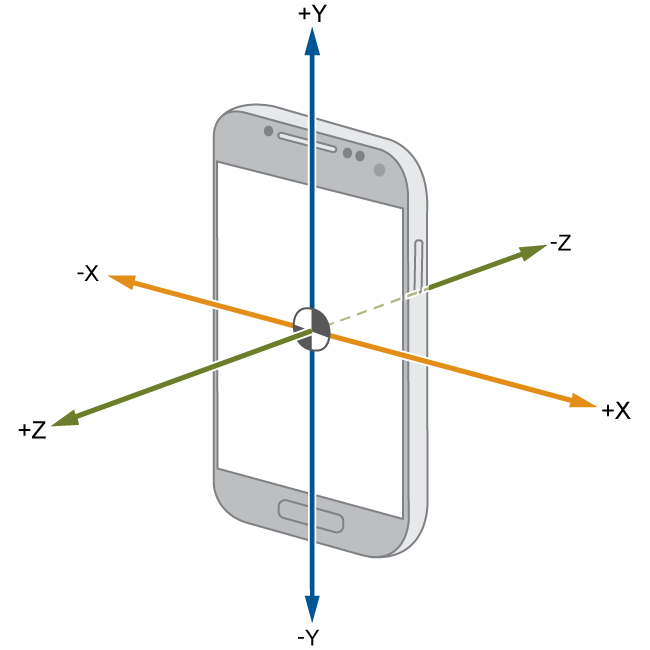
\includegraphics[width=0.4\linewidth]{img/orientation_tel.png}
    \caption{Orientation des axes sur un téléphone portable}
    \label{orientation_axes}
\end{figure}

\subsection{Accéléromètre}
Commençons par examiner les données d'accéléromètre, qui mesurent l'accélération dans les trois axes (X, Y, Z). Voici un aperçu de ces données :

\begin{figure}[h]
    \centering
    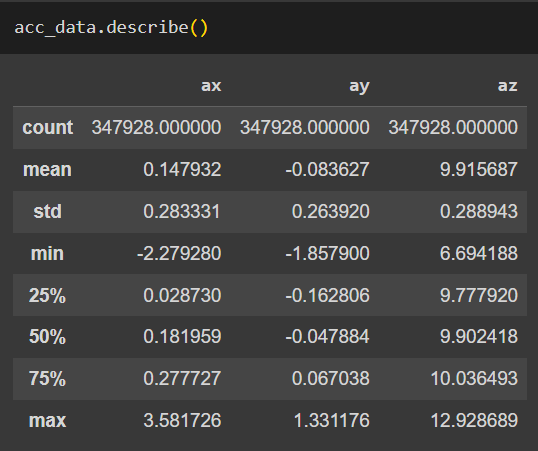
\includegraphics[width=0.4\linewidth]{img/accdata.png}
    \caption{Statistiques sommaires des données accélérométriques}
    \label{acceleration_stats}
\end{figure}

Nous pouvons observer les statistiques descriptives telles que la moyenne, l'écart-type, les valeurs minimales et maximales pour chaque axe. Cela nous donne une idée de la variabilité des données d'accélération.

\subsubsection{Graphiques d'Accélération}
Pour mieux visualiser les données d'accélération, nous avons créé des graphiques. Voici un exemple de graphique montrant l'accélération dans les trois axes au fil du temps :

\begin{figure}[h]
    \centering
    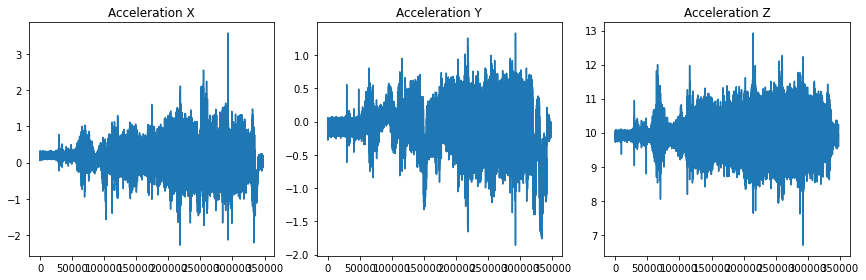
\includegraphics[width=0.8\linewidth]{img/accdata_evol.png}
    \caption{Graphique d'accélération au fil du temps}
    \label{acceleration_graph}
\end{figure}

\subsection{Données GPS}
En parallèle, nous avons également collecté des données GPS pour suivre la position du robot véhicule. Voici un aperçu de ces données :

\begin{figure}[h]
    \centering
    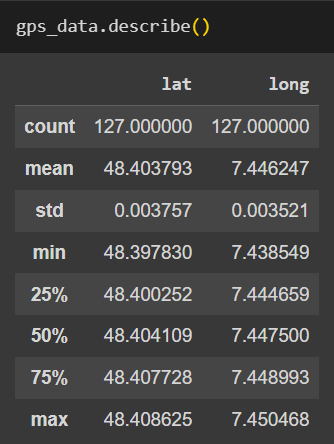
\includegraphics[width=0.3\linewidth]{img/gpsdata.png}
    \caption{Statistiques sommaires des données GPS}
    \label{gps_stats}
\end{figure}

Nous pouvons voir des statistiques sommaires pour les données GPS, nous donnant une idée des valeurs minimales et maximales des coordonnées GPS.

\subsection{Tests et Nettoyage des Données}
Enfin, nous avons effectué des tests pour évaluer la qualité des données collectées. Nous avons détecté et identifié des fichiers de données potentiellement invalides en fonction du nombre de lignes. Tout fichier contenant moins de 1500 lignes a été signalé pour un examen ultérieur.

Cette analyse préliminaire des données est cruciale pour comprendre la nature de nos enregistrements et pour préparer le terrain en vue de la création du jeu de données et de l'implémentation des modèles.
